\documentclass[]{book}
\usepackage{lmodern}
\usepackage{amssymb,amsmath}
\usepackage{ifxetex,ifluatex}
\usepackage{fixltx2e} % provides \textsubscript
\ifnum 0\ifxetex 1\fi\ifluatex 1\fi=0 % if pdftex
  \usepackage[T1]{fontenc}
  \usepackage[utf8]{inputenc}
\else % if luatex or xelatex
  \ifxetex
    \usepackage{mathspec}
  \else
    \usepackage{fontspec}
  \fi
  \defaultfontfeatures{Ligatures=TeX,Scale=MatchLowercase}
\fi
% use upquote if available, for straight quotes in verbatim environments
\IfFileExists{upquote.sty}{\usepackage{upquote}}{}
% use microtype if available
\IfFileExists{microtype.sty}{%
\usepackage[]{microtype}
\UseMicrotypeSet[protrusion]{basicmath} % disable protrusion for tt fonts
}{}
\PassOptionsToPackage{hyphens}{url} % url is loaded by hyperref
\usepackage[unicode=true]{hyperref}
\hypersetup{
            pdftitle={Burden of Disease Assessment: A Practical Guide},
            pdfauthor={Brecht Devleesschauwer},
            pdfborder={0 0 0},
            breaklinks=true}
\urlstyle{same}  % don't use monospace font for urls
\usepackage{natbib}
\bibliographystyle{apalike}
\usepackage{longtable,booktabs}
% Fix footnotes in tables (requires footnote package)
\IfFileExists{footnote.sty}{\usepackage{footnote}\makesavenoteenv{long table}}{}
\usepackage{graphicx,grffile}
\makeatletter
\def\maxwidth{\ifdim\Gin@nat@width>\linewidth\linewidth\else\Gin@nat@width\fi}
\def\maxheight{\ifdim\Gin@nat@height>\textheight\textheight\else\Gin@nat@height\fi}
\makeatother
% Scale images if necessary, so that they will not overflow the page
% margins by default, and it is still possible to overwrite the defaults
% using explicit options in \includegraphics[width, height, ...]{}
\setkeys{Gin}{width=\maxwidth,height=\maxheight,keepaspectratio}
\IfFileExists{parskip.sty}{%
\usepackage{parskip}
}{% else
\setlength{\parindent}{0pt}
\setlength{\parskip}{6pt plus 2pt minus 1pt}
}
\setlength{\emergencystretch}{3em}  % prevent overfull lines
\providecommand{\tightlist}{%
  \setlength{\itemsep}{0pt}\setlength{\parskip}{0pt}}
\setcounter{secnumdepth}{5}
% Redefines (sub)paragraphs to behave more like sections
\ifx\paragraph\undefined\else
\let\oldparagraph\paragraph
\renewcommand{\paragraph}[1]{\oldparagraph{#1}\mbox{}}
\fi
\ifx\subparagraph\undefined\else
\let\oldsubparagraph\subparagraph
\renewcommand{\subparagraph}[1]{\oldsubparagraph{#1}\mbox{}}
\fi

% set default figure placement to htbp
\makeatletter
\def\fps@figure{htbp}
\makeatother

\usepackage{booktabs}
\usepackage{amsthm}
\makeatletter
\def\thm@space@setup{%
  \thm@preskip=8pt plus 2pt minus 4pt
  \thm@postskip=\thm@preskip
}
\makeatother

\title{Burden of Disease Assessment: A Practical Guide}
\author{Brecht Devleesschauwer}
\date{2020-05-26}

\begin{document}
\maketitle

{
\setcounter{tocdepth}{1}
\tableofcontents
}
\chapter*{Preface}\label{preface}
\addcontentsline{toc}{chapter}{Preface}

Disability-Adjusted Life Years (DALYs) have become a key indicator in
descriptive epidemiology. DALYs represent the number of healthy life
years lost due to ill health and mortality, and allow comparing the
population health impact of diseases, injuries and risk factors.

Although the DALY concept has been introduced nearly 30 years ago, there
is still little guidance available on their calculation. This book aims
to address this gap, through a combination of theoretical sections,
simplified examples, and real-life experiences.

This book is the result of interactions and collaborations within the
European Burden of Disease Network (COST Action CA18218), supported by
COST (cooperation in science and technology). Further information on the
network is available via \url{https://www.burden-eu.net}.

\section*{Why read this book}\label{why-read-this-book}
\addcontentsline{toc}{section}{Why read this book}

This book is primarily intended for students, researchers and public
health professionals interested in learning how to calculate DALYs.

However, it should also be noted that the \textbf{best way of learning
is by doing}. We therefore hope that this book can encourage you to get
started with your own calculation examples.

\section*{Structure of the book}\label{structure-of-the-book}
\addcontentsline{toc}{section}{Structure of the book}

The first part of the book is dedicated to the basic concepts of DALY
calculations. Starting from simple examples, different layers of
complexity will be introduced.

The second part of the book is dedicated to national burden of disease
studies.

\chapter*{About the authors}\label{about-the-authors}
\addcontentsline{toc}{chapter}{About the authors}

\section*{Brecht Devleesschauwer}\label{brecht-devleesschauwer}
\addcontentsline{toc}{section}{Brecht Devleesschauwer}

Some info here.

\url{https://twitter.com/brechtdv}

\part*{Part I: Calculating
DALYs}\label{part-part-i-calculating-dalys}
\addcontentsline{toc}{part}{Part I: Calculating DALYs}

\chapter{Introduction}\label{introduction}

The ultimate goal of public health policy is to protect and promote the
population's health (Devleesschauwer et al., 2014a). This requires
information on the health status of the population, often referred to as
the ``burden of disease''. In order to make relevant decisions and set
appropriate priorities, policy makers need to be informed about the size
of health problems in the population, the groups that are particularly
at risk, and the trends in the state of health over time. In addition,
an accurate estimate of the population's health status can be used for
determining the expected health care use and is vital for prioritizing
effective interventions and evaluating their impact and
cost-effectiveness (Tan-Torres Edejer et al., 2003).

As public health is a multifactorial phenomenon with many facets, the
disease burden of the population can be described by a variety of
indicators. Typical indicators of population health are life expectancy,
cause-specific mortality rates, numbers of new and existing cases of
specific diseases (i.e., incidence and prevalence), perceived health,
the occurrence of physical and mental limitations and disability, but
also more indirect measures, such as absenteeism, incapacity of work,
and the use of medical facilities and the associated costs. However, all
these indicators highlight only one facet of public health, i.e., either
mortality or morbidity.

Summarizing public health in terms of mortality-based indicators, such
as life expectancy, dates from the time when only reliable data for
mortality existed. In many countries, however, one has been confronted
with ageing populations and an epidemiological transition of public
health problems. The importance of early mortality due to plagues and
famines has been replaced by chronic, non-communicable diseases, while
communicable diseases remain a real threat, causing a ``double burden''
(Marshall, 2004). Cardiovascular diseases and cancers have replaced
infectious diseases as the main causes of death. However, these diseases
are also associated with an important morbidity component, due to the
life prolonging effect of continuously improving medical practice
(Jelenc et al., 2012). Moreover, not only an extended life expectancy
per se is aimed for, living these extra years in good health has become
just as important (Bryant et al., 2001). As a result, current health
policy requires a global overview of public health, one that combines
morbidity and mortality and takes account of health-related quality of
life (Robine et al. 2013).

Given the importance of combining morbidity and mortality, several
summary measures of population health (SMPH) have been proposed and
implemented (Murray et al., 2000; Table 1). SMPHs may be divided into
two broad families: health expectancies or experiences and health gaps,
but all have in common that they use ``time'' as the common measure for
quantifying health or health loss. The most powerful SMPHs are those
that are able to combine morbidity and mortality into a single figure.

\begin{longtable}[]{@{}lll@{}}
\caption{(\#smph) Classification of summary measures of population
health}\tabularnewline
\toprule
\begin{minipage}[b]{0.08\columnwidth}\raggedright\strut
\strut
\end{minipage} & \begin{minipage}[b]{0.50\columnwidth}\raggedright\strut
Health Experience\strut
\end{minipage} & \begin{minipage}[b]{0.34\columnwidth}\raggedright\strut
Health Gap\strut
\end{minipage}\tabularnewline
\midrule
\endfirsthead
\toprule
\begin{minipage}[b]{0.08\columnwidth}\raggedright\strut
\strut
\end{minipage} & \begin{minipage}[b]{0.50\columnwidth}\raggedright\strut
Health Experience\strut
\end{minipage} & \begin{minipage}[b]{0.34\columnwidth}\raggedright\strut
Health Gap\strut
\end{minipage}\tabularnewline
\midrule
\endhead
\begin{minipage}[t]{0.08\columnwidth}\raggedright\strut
Mortality\strut
\end{minipage} & \begin{minipage}[t]{0.50\columnwidth}\raggedright\strut
Life Expectancy\strut
\end{minipage} & \begin{minipage}[t]{0.34\columnwidth}\raggedright\strut
Potential Years of Life Lost(Years of Potential Life Lost)Standard
Expected Years of Life Lost\strut
\end{minipage}\tabularnewline
\begin{minipage}[t]{0.08\columnwidth}\raggedright\strut
Morbidity\strut
\end{minipage} & \begin{minipage}[t]{0.50\columnwidth}\raggedright\strut
Quality-Adjusted Life Year\strut
\end{minipage} & \begin{minipage}[t]{0.34\columnwidth}\raggedright\strut
Years Lived with Disability\strut
\end{minipage}\tabularnewline
\begin{minipage}[t]{0.08\columnwidth}\raggedright\strut
Morbidity \& Mortality\strut
\end{minipage} & \begin{minipage}[t]{0.50\columnwidth}\raggedright\strut
Active Life ExpectancyDisability-Free Life ExpectancyHealthy Life
YearsQuality-Adjusted Life ExpectancyDisability-Adjusted Life
Expectancy\strut
\end{minipage} & \begin{minipage}[t]{0.34\columnwidth}\raggedright\strut
Disability-Adjusted Life Year\strut
\end{minipage}\tabularnewline
\bottomrule
\end{longtable}

Driven by the influential Global Burden of Disease (GBD) projects
initiated in the early 1990s (Murray and Lopez, 1996), the
Disability-Adjusted Life Year (DALY) has become the dominant SMPH for
quantifying burden of disease. The DALY metric has therefore been
selected as key SMPH for the Belgian National Burden of Disease study.
DALYs measure the health gap from a life lived in perfect health, and
quantify this health gap as the number of healthy life years lost due to
morbidity and mortality. Although the basic DALY formulas are rather
straightforward, the calculation of DALYs, like any other SMPH, requires
several assumptions, some of which are not always obvious. Furthermore,
DALY-based burden of disease studies are almost always confronted by
uncertainties and almost always require manipulations of epidemiological
data.

\chapter{Basic concepts}\label{basic-concepts}

\chapter{Data needs}\label{data-needs}

\chapter{Disability weights}\label{disability-weights}

\chapter{Comorbidity}\label{comorbidity}

\chapter{Residual life expectancy}\label{residual-life-expectancy}

\chapter{Quantifying uncertainty}\label{quantifying-uncertainty}

\section{Sources of uncertainty}\label{sources-of-uncertainty}

Nearly every DALY estimation is subject to data uncertainty and
modelling choices. The resulting DALY estimate is thus hardly ever a
single, fixed value, defined with perfect accuracy and precision. In a
practical guide on accounting for uncertainty in decision-analytic
models, Bilcke et al. (2011) classified uncertainty into three
categories: parameter uncertainty (uncertainty regarding the true value
of the model parameters); structural or model uncertainty (uncertainty
regarding the model structure); and methodological uncertainty
(uncertainty due to normative or subjective modelling choices).

\subsection{Parameter uncertainty}\label{parameter-uncertainty}

Parameter uncertainty relates to a lack of knowledge on the true value
of model parameters. DALY calculations require demographic,
epidemiological, and severity parameters, each of which can be
uncertain. Severity parameters, such as duration and disability weight,
relate to individual patients and can therefore also be variable.
Variability, sometimes referred to as stochasticity or first order
uncertainty, distinguishes itself from uncertainty in that it is an
inherent property of populations, and cannot be reduced by gaining more
information, e.g., by increasing the sample size.

In general, parameter uncertainty results from sampling error and/or
systematic error or bias. Sampling error is well known and well-studied
by statisticians. It arises when a parameter is inferred from a
representative sample of the population of interest. It can be modelled
directly, for instance by assuming a Binomial distribution for a
prevalence estimate obtained by testing a certain population sample. At
a different level, when parameters are modelled from a statistical
model, the resulting standard errors also reflect this sampling error.
Systematic error, on the other hand, is less well-studied, but is
potentially much more important. In DALY calculations, systematic error
is very often related to the extrapolation of parameter values from
non-representative populations or time periods. The most extreme form of
extrapolation occurs when there is a complete lack of data, a common
situation in global or regional burden of disease studies. It is not
clear to what extent these alternative settings are representative for
the concerned setting, and different alternative settings may provide
different parameter values, related to different levels of bias.
Ill-defined coding, misclassification and underestimation are typical
and common sources of systematic error in epidemiological parameters
such as prevalence, incidence and mortality (see section 3.1).

A specific problem related to parameter uncertainty arises when
uncertainty is correlated. This may be the case if DALYs are calculated
per age and sex group, but parameters are only available at a less
granular level. In GBD studies, this problem occurs when regional or
global parameters are used instead of country-specific parameters and
applied to each of the concerned countries. Such issues may be described
as stratification uncertainty: uncertainty arising because the level of
detail required in the DALY calculations does not match the level of
stratification in the data (Devleesschauwer et al., 2016).

\subsection{Model uncertainty}\label{model-uncertainty}

DALY calculations follow a disease model or outcome tree, i.e., a
schematic representation of health states that are causally related to
the risk factor, hazard or disease of interest (Devleesschauwer et al.,
2014c). Uncertainty in this disease model may arise when there is
insufficient or conflicting evidence on the causal relation of certain
symptoms. Such uncertainty is common for long-term outcomes of
infections, such as cirrhosis and hepatocellular carcinoma following
hepatitis C and B infection (García-Fulgueiras et al., 2011), or
post-infectious irritable bowel syndrome following giardiosis (Havelaar
et al., 2012). Model uncertainty in DALY calculations may also originate
from health states being controversial due to ethical reservations. In
this respect, Jamison et al. (2006) discussed the inclusion of
stillbirths in GBD assessments.

A second source of model uncertainty can be linked to the
epidemiological data used in the DALY calculations. Often the available
data come with a lot of restrictions, and several assumptions need to be
made to transform these into useable numbers. Whether or not data should
be corrected for underreporting or misclassification may for instance
become a source of model uncertainty.

\subsection{Methodological
uncertainty}\label{methodological-uncertainty}

The DALY metric encapsulates various methodological choices, often
referred to as value choices. All of these choices are normative and
thus subjective, as there is no intrinsically correct choice. As a
result, different choices are being made, and contested, in literature.

The different methodological choices that need to be made when
calculating DALYs have been outlined in section 2 of the manual. Here we
provide some examples of how these choices can lead to uncertainties.

\begin{enumerate}
\def\labelenumi{(\arabic{enumi})}
\tightlist
\item
  YLD perspective
\end{enumerate}

The GBD 2010 study introduced a prevalence-based version of the YLD,
defined as the product of number of prevalent cases and DW (Murray et
al., 2012). Both perspectives are equally valid, but have a different
interpretation. The choice between an incidence and prevalence
perspective therefore remains a normative choice.

\begin{enumerate}
\def\labelenumi{(\arabic{enumi})}
\setcounter{enumi}{1}
\tightlist
\item
  Disability weights
\end{enumerate}

Different methods exist for deriving DWs, based on either an econometric
or psychometric philosophical perspective on health-related quality of
life (Haagsma et al., 2014; Rehm and Frick, 2010). Also, subjective
choices need to be made on which population's values to use: those of
patients, lay people, or disease experts? Phanthunane et al. (2010) for
instance compared DWs for schizophrenia elicited from both patients and
clinicians using different multi-attribute utility instruments.
Furthermore, DWs may be corrected for comorbidity, but again, different
methods have been proposed, ranging from the use of arbitrary
attribution factors (Mathers et al., 2000), over maximum limit or
multiplicative approaches (Mathers et al., 2001; Murray et al., 2012),
to regression models (Cuijpers et al., 2011; Lokkerbol et al., 2013).
Finally, when DWs are not available for specific health states,
``proxy'' DWs are commonly derived by mapping the concerned health state
to alternative health states for which DWs are available. LaBeaud et al.
(2011) for instance present a set of proxy DWs for arbovirus-related
long-term sequelae, showing the uncertainty induced by the need to map
to analogous health states.

\begin{enumerate}
\def\labelenumi{(\arabic{enumi})}
\setcounter{enumi}{2}
\tightlist
\item
  Residual life expectancy table
\end{enumerate}

Different possibilities exist regarding the choice of the life
expectancy table. The use of local (e.g., national) life expectancy
tables has been propagated to reflect the local epidemiological
situation (Plass et al., 2013). Local life expectancy tables have also
been used for specific population subgroups, such as ethnic minorities
in Australia (Costilla et al., 2013), or for future populations, such as
the French population in 2020 (Lapostolle et al., 2008). Some authors
further adapted local life expectancies to reflect reduced life
expectancy in fatal cases, assuming that these cases had underlying
diseases (Wielders et al., 2012). Matemba et al. (2010) used the
opposite approach, by adapting the local life expectancy table to
estimate the burden of sleeping sickness if the HIV/aids epidemic had
not occurred. In addition to these local life expectancy tables, the use
of so-called ``standard'' life expectancy tables has been promoted to
ensure comparability across populations. To date, however, there are
three different ``standard'' life expectancy tables in use (Appendix A).

\begin{enumerate}
\def\labelenumi{(\arabic{enumi})}
\setcounter{enumi}{3}
\tightlist
\item
  Social weighting
\end{enumerate}

The basic DALY formulas can be extended by including age weighting and
time discounting functions (Devleesschauwer et al., 2014b). Whether or
not these social weighting functions should be used remains a subjective
choice, and has indeed been the subject of debate (Barendregt et al.,
1996). Furthermore, there is no consensus on the exact parameterization
of these social weighting functions. Although age weighting commonly
follows the original formulation, some authors proposed alternative
formulations that better reflected their local situation (Yang et al.,
2004). When discounting time, the standard choice has been to apply a
3\% discount rate, but certain national instances propose different
weights, e.g., 1.5\% in The Netherlands and 3.5\% in the United Kingdom
(Havelaar et al., 2012).

\section{Dealing with uncertainties}\label{dealing-with-uncertainties}

\subsection{Probabilistic sensitivity
analysis}\label{probabilistic-sensitivity-analysis}

By far the most powerful method to deal with parameter uncertainty is
probabilistic sensitivity analysis (PSA), sometimes also called
uncertainty analysis or uncertainty propagation. In PSA, the uncertain
parameters are represented by uncertainty distributions, thereby
following the Bayesian definition of probability as a degree of belief
instead of a long-term frequency. PSA uses Monte Carlo simulations, or
parametric bootstrap, to sample random values from the specified
uncertainty distributions (Fig 7). At each iteration, the sampled values
are used to calculated a DALY estimate. The combination of iterations
therefore results in an empirical distribution of DALY estimates,
reflecting the joint uncertainty in the input parameters (Fig 8). This
resulting distribution can be summarized by its mean and a 95\%
uncertainty interval defined as the 2.5th and 97.5th percentile. PSA is
typically used to propagate uncertainty, thereby ignoring variability.
Nevertheless, it would be possible to simulate both processes using
second order or two-dimensional Monte Carlo simulations (Havelaar et
al., 2004).

Fig 7. Monte Carlo simulation. Top: red dots represent seven simulated
values from a normal(0;1) distribution. Bottom: as the number of Monte
Carlo simulations increases, the histogram of simulated values becomes
an increasingly better approximation of the target distribution (in
blue).

\begin{figure}
\centering
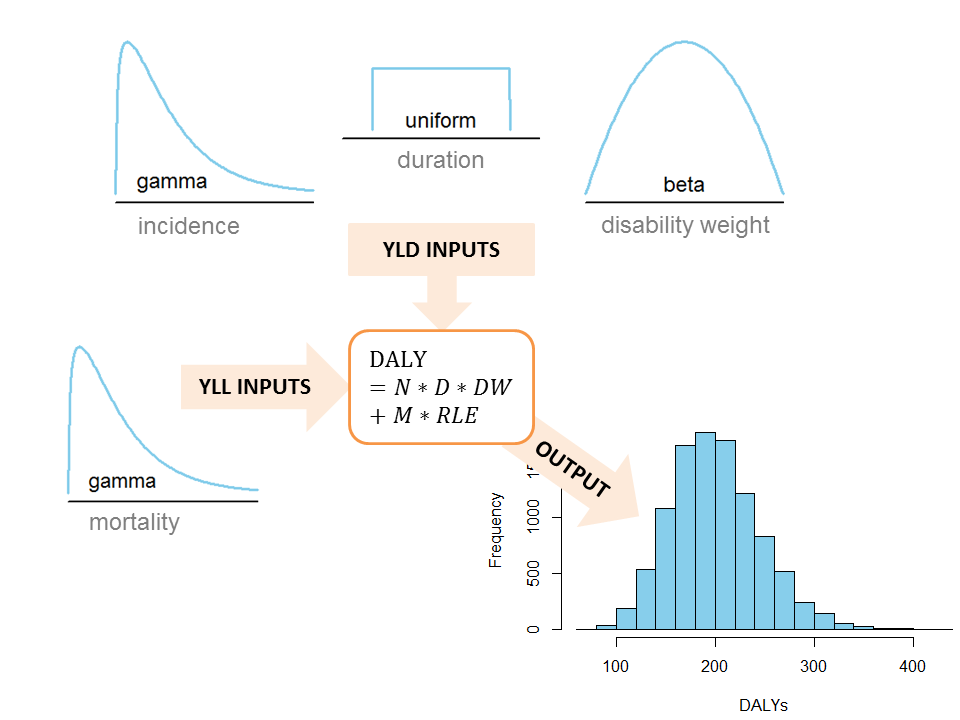
\includegraphics{img/uncertainty.png}
\caption{Probabilistic sensitivity analysis applied to DALY
calculations. Probability distributions are specified to reflect the
uncertainty in the input parameters; random values are simulated from
these distributions and used to calculate DALYs, resulting in an
empirical distribution of the joint uncertainty in the DALY estimate.}
\end{figure}

\subsection{Variable importance
analysis}\label{variable-importance-analysis}

To evaluate which uncertain parameters contribute most to the
uncertainty in the final DALY estimate, variable importance analysis
techniques can be applied. These techniques are often also called
sensitivity analyses, adding to the confusion. A common approach is to
calculate standardized regression coefficients, by regressing the
standardized input parameters against the (standardized) simulated DALYs
obtained with PSA (Verhoef et al., 2012). The resulting regression
coefficients reflect the expected (standard deviation) change in DALY
per standard deviation change in the respective input parameter.
Alternatively, partial correlation coefficients may be calculated, which
do not assume a linear relationship between inputs and output. For both
methods, the resulting variable importance coefficients may be
represented in a tornado graph, which sorts, from top to bottom, the
input variables in order of their importance (Fig 9).

Fig 9. Tornado graph showing the results of a variable importance
analysis in a study on the burden of neurocysticercosis-epilepsy in
Tanzania (Trevisan et al. 2016). E: epilepsy; NCC: neurocysticercosis.

\subsection{Scenario analyses}\label{scenario-analyses}

Scenario analyses imply that DALYs are calculated under different
assumptions and compared. These analyses are the method of choice for
quantifying model and methodological uncertainty. Fig 10 shows an
example.

Fig 10. Scenario analysis of the disease burden of toxoplasmosis in the
Netherlands (Havelaar et al., 2007). The evaluated scenarios include
alternative incidence data, the inclusion of time discounting, the
exclusion of fetal losses, and the use of alternative disability weights

In theory, model and methodological uncertainty may also be assessed
through PSA, by parameterizing the uncertain model elements or the
methodological choices. Whether or not underreporting should be
corrected for, could for instance be parameterized by specifying an
uncertainty distribution on the underreporting factor with a minimum of
one and a certain maximum. Indeed, Luz et al. (2009) performed a PSA
with a multiplication factor ranging from 0.3 to 10, thus accounting for
over-reporting, over correct reporting, to underreporting, with a
stronger emphasis on the former. Including or excluding a certain health
state could for instance be modelled as a Bernoulli random variable with
inclusion probability π. The resulting distribution of simulated DALY
estimates will then be a combination of different disease model
assumptions, which in itself can be regarded as a new scenario.
Furthermore, parameterization would prevent decision makers to identify
the results that correspond to their model choice or methodological
preference.

\part*{Part 2: From Theory to
Practice}\label{part-part-2-from-theory-to-practice}
\addcontentsline{toc}{part}{Part 2: From Theory to Practice}

\chapter{Disease models}\label{disease-models}

\chapter{Infectious diseases}\label{infectious-diseases}

\chapter{Injuries}\label{injuries}

\chapter{Risk factors}\label{risk-factors}

\part*{Part III: National Burden of Disease
Studies}\label{part-part-iii-national-burden-of-disease-studies}
\addcontentsline{toc}{part}{Part III: National Burden of
Disease Studies}

\chapter{Planning and organization}\label{planning-and-organization}

\chapter{Ill-defined deaths}\label{ill-defined-deaths}

\chapter{Healthy life expectancy}\label{healthy-life-expectancy}

\chapter{Knowledge translation}\label{knowledge-translation}

\bibliography{book.bib,packages.bib}

\end{document}
